% !TEX program = lualatex
        
% IMPORTANT! In order for the document to compile, one needs to use XeLaTeX or LuaLaTeX as compiler. This can be done in  Overleaf by Menu -> Settings -> Compiler -> Choose XeLaTeX/LuaLaTeX
\documentclass[t,24pt,aspectratio=169]{beamer}

\usepackage{UAM}
\usepackage{multicol} % Package for multiple coloumns
\usepackage[style=authoryear]{biblatex}
\usepackage{listings}
\usepackage{xcolor}

\definecolor{codegreen}{rgb}{0,0.6,0}
\definecolor{codegray}{rgb}{0.5,0.5,0.5}
\definecolor{codepurple}{rgb}{0.58,0,0.82}
\definecolor{backcolour}{rgb}{0.95,0.95,0.92}

\lstset{
	backgroundcolor=\color{backcolour},
	commentstyle=\color{codegreen},
	keywordstyle=\color{magenta},
	numberstyle=\tiny\color{codegray},
	stringstyle=\color{codepurple},
	basicstyle=\ttfamily\footnotesize,
	breaklines=true,
	frame=single,
	showstringspaces=false
}

%\usepackage{minted}
% lualatex -shell-escape -synctex=1 -interaction=nonstopmode archivo.tex

% \toplinje{Text at top} % The text at top. Remove the command if no text is desired


\addbibresource{references.bib}
\begin{document}

% The first slide. One can for instance change the main title, the subtitle, speaker, KU-unit, date and backgroundimage
{
\setbeamertemplate{background}{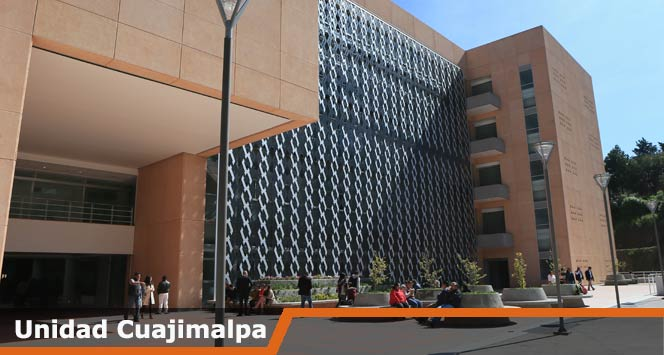
\includegraphics[width=\paperwidth,height=\paperheight]{uam/cua_05.jpg}}
\begin{frame}
    \begin{textblock*}{\textwidth}(0.53\textwidth,0.1\textheight)
        \begin{beamercolorbox}[wd=8.5cm,ht=7.3cm,sep=0.5cm]{hvidbox}
            \fontsize{5}{10}\fontfamily{ptm}\selectfont \textls[200]{UNIVERSIDAD AUTÓNOMA METROPOLITANA}
            \noindent\textcolor{KUrod}{\rule{6.8cm}{0.4pt}}
        \end{beamercolorbox}
    \end{textblock*}
    \begin{textblock*}{\textwidth}(0.53\textwidth,0.1\textheight)
        \begin{beamercolorbox}[wd=8.5cm,sep=0.5cm]{hvidbox}
                \Huge \textcolor{KUrod}{Integración de sistemas}
                \vspace{0.5cm}
                \par
                \Large Panorama histórico y concepto actual de integración

                \vspace{0.5cm}
                \par
                \normalsize Juan Alvarado
        \end{beamercolorbox}
    \end{textblock*}
    \begin{textblock}{1}(14.5,11.38)
        % \includegraphics[width=1cm]{KU/KU-logo.png}
    \end{textblock}
\end{frame}
}


        %%%%%%%%%%%%%%%%%%%%%%%%%%%%%%%%%%%%%%%
	\begin{frame}[fragile, hvid]
		\frametitle{Punto a punto: el “cableado spaghetti”}
			\vfill
			\centering
			\Huge{Punto a punto: el “cableado spaghetti”}
			\vfill
	\end{frame}
%%%%%%%%%%%%%%%%%%%%%%%%%%%%%%%%%%%%%%%


%%%%%%%%%%%%%%%%%%%%%%%%%%%%%%%%%%%%%%%
	\begin{frame}[fragile, hvid]
		\frametitle{Punto a punto: el “cableado spaghetti”}
			\vfill
La integración punto a punto fue la forma dominante de conectar sistemas en los primeros años de la informática empresarial.
\\~\\
			\vfill
	\end{frame}
%%%%%%%%%%%%%%%%%%%%%%%%%%%%%%%%%%%%%%%


%%%%%%%%%%%%%%%%%%%%%%%%%%%%%%%%%%%%%%%
	\begin{frame}[fragile, hvid]
		\frametitle{Punto a punto: el “cableado spaghetti”}
			\vfill
Consistía en que cada par de aplicaciones que necesitaba hablar entre sí establecía su propio canal de comunicación con protocolos y formatos hechos a la medida.
\\~\\
			\vfill
	\end{frame}
%%%%%%%%%%%%%%%%%%%%%%%%%%%%%%%%%%%%%%%


%%%%%%%%%%%%%%%%%%%%%%%%%%%%%%%%%%%%%%%
	\begin{frame}[fragile, hvid]
		\frametitle{Punto a punto: el “cableado spaghetti”}
			\vfill
\begin{multicols}{2} 

Cada vez que aparecía un nuevo sistema, se agregaban más conexiones directas, lo que generaba una red cada vez más compleja y difícil de mantener.
\\~\\
\columnbreak
\centering

\includegraphics[width=6.6cm,height=5.9cm,keepaspectratio]{img/mark-995567_640.jpeg}
\end{multicols}
			\vfill
	\end{frame}
%%%%%%%%%%%%%%%%%%%%%%%%%%%%%%%%%%%%%%%


%%%%%%%%%%%%%%%%%%%%%%%%%%%%%%%%%%%%%%%
	\begin{frame}[fragile, hvid]
		\frametitle{Punto a punto: el “cableado spaghetti”}
			\vfill
\begin{multicols}{2} 

En organizaciones grandes esto producía un efecto “spaghetti”: muchas conexiones cruzadas, lógica de integración duplicada y alta dependencia entre sistemas.
\\~\\
Cambiar o reemplazar una aplicación se volvía costoso, porque había que reescribir múltiples integraciones.
\\~\\
\columnbreak
\centering

\includegraphics[width=6.6cm,height=5.9cm,keepaspectratio]{img/pexels-pixabay-60504.jpg}
\end{multicols}
			\vfill
	\end{frame}
%%%%%%%%%%%%%%%%%%%%%%%%%%%%%%%%%%%%%%%


%%%%%%%%%%%%%%%%%%%%%%%%%%%%%%%%%%%%%%%
	\begin{frame}[fragile, hvid]
		\frametitle{Punto a punto: el “cableado spaghetti”}
			\vfill
\textbf{Actividad – Mapa de spaghetti}
\\~\\
En equipos de 3–4, elijan un escenario sencillo y que dibujen en pizarrón (no borrar) las conexiones punto a punto entre sistemas si cada par se conecta directamente.
\\~\\
			\vfill
	\end{frame}
%%%%%%%%%%%%%%%%%%%%%%%%%%%%%%%%%%%%%%%


%%%%%%%%%%%%%%%%%%%%%%%%%%%%%%%%%%%%%%%
	\begin{frame}[fragile, hvid]
		\frametitle{Punto a punto: el “cableado spaghetti”}
			\vfill
\begin{multicols}{2} 

Después, cada equipo identifica:
\\~\\
- Cuántas integraciones habría si se agregan nuevos sistemas (por ejemplo, CRM, app móvil).
\\~\\
- Qué pasaría si se cambia el sistema de pagos.
\\~\\
Discutir brevemente cómo crece la complejidad en función del número de sistemas.
\\~\\
\columnbreak
\centering

\includegraphics[width=6.6cm,height=5.9cm,keepaspectratio]{img/mark-995567_640.jpeg}
\end{multicols}
			\vfill
	\end{frame}
%%%%%%%%%%%%%%%%%%%%%%%%%%%%%%%%%%%%%%%


%%%%%%%%%%%%%%%%%%%%%%%%%%%%%%%%%%%%%%%
	\begin{frame}[fragile, hvid]
		\frametitle{SOA: servicios y buses de integración}
			\vfill
			\centering
			\Huge{SOA: servicios y buses de integración}
			\vfill
	\end{frame}
%%%%%%%%%%%%%%%%%%%%%%%%%%%%%%%%%%%%%%%


%%%%%%%%%%%%%%%%%%%%%%%%%%%%%%%%%%%%%%%
	\begin{frame}[fragile, hvid]
		\frametitle{SOA: servicios y buses de integración}
			\vfill
\begin{multicols}{2} 

Para reducir el caos de las integraciones punto a punto surgió la Arquitectura Orientada a Servicios (SOA).
\\~\\
\columnbreak
\centering

\includegraphics[width=6.6cm,height=5.9cm,keepaspectratio]{img/exclamation-mark-blue.png}
\end{multicols}
			\vfill
	\end{frame}
%%%%%%%%%%%%%%%%%%%%%%%%%%%%%%%%%%%%%%%


%%%%%%%%%%%%%%%%%%%%%%%%%%%%%%%%%%%%%%%
	\begin{frame}[fragile, hvid]
		\frametitle{SOA: servicios y buses de integración}
			\vfill
\begin{multicols}{2} 

En SOA, la lógica de negocio se agrupa en servicios bien definidos que representan capacidades (por ejemplo, “Servicio de Clientes”, “Servicio de Facturación”), en lugar de conexiones ad hoc entre aplicaciones.
\\~\\
\columnbreak
\centering

\includegraphics[width=6.6cm,height=5.9cm,keepaspectratio]{img/pexels-pixabay-247791.jpg}
\end{multicols}
			\vfill
	\end{frame}
%%%%%%%%%%%%%%%%%%%%%%%%%%%%%%%%%%%%%%%


%%%%%%%%%%%%%%%%%%%%%%%%%%%%%%%%%%%%%%%
	\begin{frame}[fragile, hvid]
		\frametitle{SOA: servicios y buses de integración}
			\vfill
\begin{multicols}{2} 

Los servicios se comunican mediante mensajes estándar y suelen utilizar un middleware de integración como un ESB (Enterprise Service Bus) para orquestar, transformar y enrutar mensajes.
\\~\\
\columnbreak
\centering
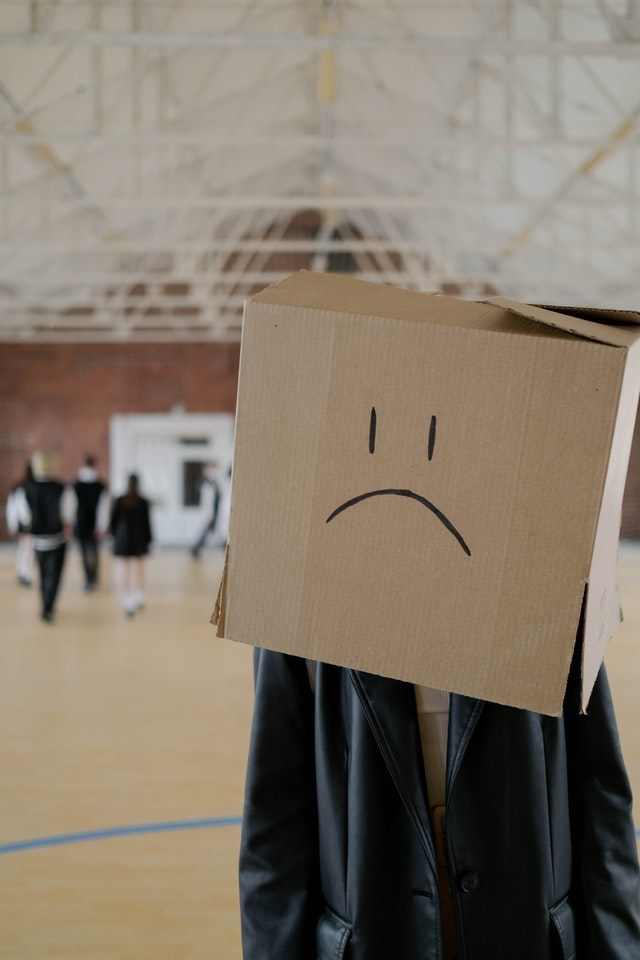
\includegraphics[width=6.6cm,height=5.9cm,keepaspectratio]{img/sad_box_face.jpg}
\end{multicols}
			\vfill
	\end{frame}
%%%%%%%%%%%%%%%%%%%%%%%%%%%%%%%%%%%%%%%


%%%%%%%%%%%%%%%%%%%%%%%%%%%%%%%%%%%%%%%
	\begin{frame}[fragile, hvid]
		\frametitle{SOA: servicios y buses de integración}
			\vfill
SOA enfatiza contratos claros entre productor y consumidor de servicios, lo que facilita la reutilización de funcionalidades en diferentes aplicaciones.
\\~\\
			\vfill
	\end{frame}
%%%%%%%%%%%%%%%%%%%%%%%%%%%%%%%%%%%%%%%


%%%%%%%%%%%%%%%%%%%%%%%%%%%%%%%%%%%%%%%
	\begin{frame}[fragile, hvid]
		\frametitle{SOA: servicios y buses de integración}
			\vfill
Sin embargo, muchas implementaciones de SOA se volvieron pesadas, con gobernanza compleja y dependencia fuerte del ESB.
\\~\\
			\vfill
	\end{frame}
%%%%%%%%%%%%%%%%%%%%%%%%%%%%%%%%%%%%%%%


%%%%%%%%%%%%%%%%%%%%%%%%%%%%%%%%%%%%%%%
	\begin{frame}[fragile, hvid]
		\frametitle{SOA: servicios y buses de integración}
			\vfill
\begin{multicols}{2} 

\textbf{Actividad – Reorganizar el spaghetti en servicios}
\\~\\
En los mismos equipos, reutilicen el escenario elegido y ya dibujado.
\\~\\
Ahora deben:
\\~\\
- Proponer de 3 a 5 servicios de negocio (por ejemplo, Clientes, Pedidos, Pagos, Inventario).
\\~\\
\columnbreak
\centering

\includegraphics[width=6.6cm,height=5.9cm,keepaspectratio]{img/pexels-cottonbro-studio-6804080.jpg}
\end{multicols}
			\vfill
	\end{frame}
%%%%%%%%%%%%%%%%%%%%%%%%%%%%%%%%%%%%%%%


%%%%%%%%%%%%%%%%%%%%%%%%%%%%%%%%%%%%%%%
	\begin{frame}[fragile, hvid]
		\frametitle{SOA: servicios y buses de integración}
			\vfill
\begin{multicols}{2} 

- Dibujar cómo los sistemas existentes (web, ERP, pasarela de pago) consumirían esos servicios en vez de conectarse entre sí directamente.
\\~\\
\columnbreak
\centering

\includegraphics[width=6.6cm,height=5.9cm,keepaspectratio]{img/pexels-cottonbro-studio-5473955.jpg}
\end{multicols}
			\vfill
	\end{frame}
%%%%%%%%%%%%%%%%%%%%%%%%%%%%%%%%%%%%%%%


%%%%%%%%%%%%%%%%%%%%%%%%%%%%%%%%%%%%%%%
	\begin{frame}[fragile, hvid]
		\frametitle{SOA: servicios y buses de integración}
			\vfill
\begin{multicols}{2} 

Contrastar el nuevo diagrama con el anterior y notar el cambio en:
\\~\\
- Número de conexiones.
\\~\\
- Facilidad para agregar un nuevo canal (por ejemplo, app móvil).
\\~\\
\columnbreak
\centering

\includegraphics[width=6.6cm,height=5.9cm,keepaspectratio]{img/angry_man.jpg}
\end{multicols}
			\vfill
	\end{frame}
%%%%%%%%%%%%%%%%%%%%%%%%%%%%%%%%%%%%%%%


%%%%%%%%%%%%%%%%%%%%%%%%%%%%%%%%%%%%%%%
	\begin{frame}[fragile, hvid]
		\frametitle{Servicios web SOAP/XML en la era SOA}
			\vfill
			\centering
			\Huge{Servicios web SOAP/XML en la era SOA}
			\vfill
	\end{frame}
%%%%%%%%%%%%%%%%%%%%%%%%%%%%%%%%%%%%%%%


%%%%%%%%%%%%%%%%%%%%%%%%%%%%%%%%%%%%%%%
	\begin{frame}[fragile, hvid]
		\frametitle{Servicios web SOAP/XML en la era SOA}
			\vfill
\begin{multicols}{2} 

En la época de auge de SOA, los servicios web basados en SOAP (Simple Object Access Protocol) y XML se convirtieron en el estándar dominante para la integración entre sistemas heterogéneos.
\\~\\
\columnbreak
\centering
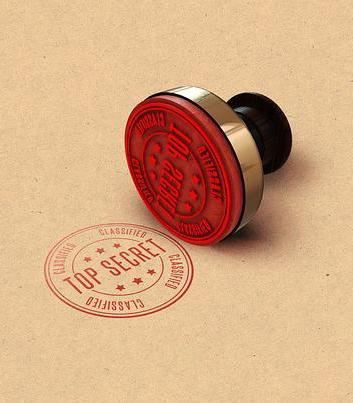
\includegraphics[width=6.6cm,height=5.9cm,keepaspectratio]{img/secret-g9ee85311d_640.jpg}
\end{multicols}
			\vfill
	\end{frame}
%%%%%%%%%%%%%%%%%%%%%%%%%%%%%%%%%%%%%%%


%%%%%%%%%%%%%%%%%%%%%%%%%%%%%%%%%%%%%%%
	\begin{frame}[fragile, hvid]
		\frametitle{Servicios web SOAP/XML en la era SOA}
			\vfill
\begin{multicols}{2} 

SOAP define un formato de mensaje estructurado en XML que viaja normalmente sobre HTTP, pero el protocolo no está limitado a HTTP.
\\~\\
\columnbreak
\centering

\includegraphics[width=6.6cm,height=5.9cm,keepaspectratio]{img/question-mark-g4c3d4d4cd_640.jpg}
\end{multicols}
			\vfill
	\end{frame}
%%%%%%%%%%%%%%%%%%%%%%%%%%%%%%%%%%%%%%%


%%%%%%%%%%%%%%%%%%%%%%%%%%%%%%%%%%%%%%%
	\begin{frame}[fragile, hvid]
		\frametitle{Servicios web SOAP/XML en la era SOA}
			\vfill
Los mensajes SOAP incluyen un sobre (Envelope) que contiene un encabezado (Header) y un cuerpo (Body), más una sección de error (Fault) cuando algo falla.
\\~\\
			\vfill
	\end{frame}
%%%%%%%%%%%%%%%%%%%%%%%%%%%%%%%%%%%%%%%


%%%%%%%%%%%%%%%%%%%%%%%%%%%%%%%%%%%%%%%
	\begin{frame}[fragile, hvid]
		\frametitle{Servicios web SOAP/XML en la era SOA}
			\vfill
Alrededor de SOAP se construyó todo un ecosistema: WSDL para describir servicios, UDDI para registrarlos y la familia de especificaciones WS-\textit{ (seguridad, confiabilidad, transacciones, etc.).
\\~\\
			\vfill
	\end{frame}
%%%%%%%%%%%%%%%%%%%%%%%%%%%%%%%%%%%%%%%


%%%%%%%%%%%%%%%%%%%%%%%%%%%%%%%%%%%%%%%
	\begin{frame}[fragile, hvid]
		\frametitle{Servicios web SOAP/XML en la era SOA}
			\vfill
Esta pila fue adoptada con fuerza en sectores como banca, gobierno y salud, donde se requerían contratos estrictos, tipos de datos muy detallados y fuertes garantías de seguridad.
\\~\\
			\vfill
	\end{frame}
%%%%%%%%%%%%%%%%%%%%%%%%%%%%%%%%%%%%%%%


%%%%%%%%%%%%%%%%%%%%%%%%%%%%%%%%%%%%%%%
	\begin{frame}[fragile, hvid]
		\frametitle{Servicios web SOAP/XML en la era SOA}
			\vfill
\begin{multicols}{2} 

\textit{(Estos temas se retomarán con más detalle en clases dedicadas a SOAP/XML, por lo que aquí solo se mencionan de manera muy general.)}
\\~\\
\columnbreak
\centering
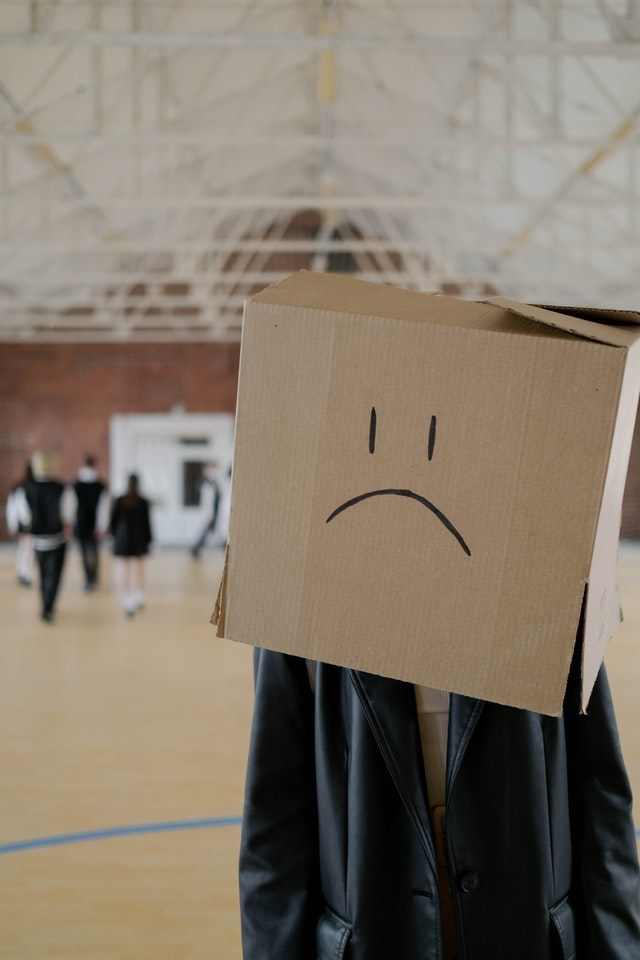
\includegraphics[width=6.6cm,height=5.9cm,keepaspectratio]{img/sad_box_face.jpg}
\end{multicols}
			\vfill
	\end{frame}
%%%%%%%%%%%%%%%%%%%%%%%%%%%%%%%%%%%%%%%


%%%%%%%%%%%%%%%%%%%%%%%%%%%%%%%%%%%%%%%
	\begin{frame}[fragile, hvid]
		\frametitle{Surgimiento de REST y las APIs modernas}
			\vfill
			\centering
			\Huge{Surgimiento de REST y las APIs modernas}
			\vfill
	\end{frame}
%%%%%%%%%%%%%%%%%%%%%%%%%%%%%%%%%%%%%%%


%%%%%%%%%%%%%%%%%%%%%%%%%%%%%%%%%%%%%%%
	\begin{frame}[fragile, hvid]
		\frametitle{Surgimiento de REST y las APIs modernas}
			\vfill
A comienzos de los 2000, Roy Fielding formuló REST (Representational State Transfer) como estilo arquitectónico para la Web, proponiendo una forma simple y uniforme de diseñar servicios usando HTTP como protocolo de aplicación.
\\~\\
			\vfill
	\end{frame}
%%%%%%%%%%%%%%%%%%%%%%%%%%%%%%%%%%%%%%%


%%%%%%%%%%%%%%%%%%%%%%%%%%%%%%%%%%%%%%%
	\begin{frame}[fragile, hvid]
		\frametitle{Surgimiento de REST y las APIs modernas}
			\vfill
REST plantea que los recursos de una aplicación se identifiquen con URIs y se manipulen con los métodos estándar de HTTP (GET, POST, PUT, DELETE, etc.).
\\~\\
			\vfill
	\end{frame}
%%%%%%%%%%%%%%%%%%%%%%%%%%%%%%%%%%%%%%%


%%%%%%%%%%%%%%%%%%%%%%%%%%%%%%%%%%%%%%%
	\begin{frame}[fragile, hvid]
		\frametitle{Surgimiento de REST y las APIs modernas}
			\vfill
\begin{multicols}{2} 

La combinación de REST con formatos ligeros como JSON hizo que las APIs fueran más fáciles de consumir desde navegadores, apps móviles y servicios en la nube.
\\~\\
\columnbreak
\centering

\includegraphics[width=6.6cm,height=5.9cm,keepaspectratio]{img/warning-g9e7961896_640.png}
\end{multicols}
			\vfill
	\end{frame}
%%%%%%%%%%%%%%%%%%%%%%%%%%%%%%%%%%%%%%%


%%%%%%%%%%%%%%%%%%%%%%%%%%%%%%%%%%%%%%%
	\begin{frame}[fragile, hvid]
		\frametitle{Surgimiento de REST y las APIs modernas}
			\vfill
\begin{multicols}{2} 

Muchas empresas de Internet (por ejemplo, redes sociales y servicios de mapas) popularizaron las APIs REST públicas, lo que impulsó aplicaciones de terceros.
\\~\\
\columnbreak
\centering

\includegraphics[width=6.6cm,height=5.9cm,keepaspectratio]{img/pexels-sora-shimazaki-5935755.jpg}
\end{multicols}
			\vfill
	\end{frame}
%%%%%%%%%%%%%%%%%%%%%%%%%%%%%%%%%%%%%%%


%%%%%%%%%%%%%%%%%%%%%%%%%%%%%%%%%%%%%%%
	\begin{frame}[fragile, hvid]
		\frametitle{Surgimiento de REST y las APIs modernas}
			\vfill
\begin{multicols}{2} 

REST no reemplazó automáticamente a SOAP, pero sí se volvió el enfoque dominante para integraciones web nuevas, sobre todo cuando se privilegian simplicidad y agilidad sobre contratos muy rígidos.
\\~\\
\columnbreak
\centering

\includegraphics[width=6.6cm,height=5.9cm,keepaspectratio]{img/pexels-cottonbro-studio-5474295.jpg}
\end{multicols}
			\vfill
	\end{frame}
%%%%%%%%%%%%%%%%%%%%%%%%%%%%%%%%%%%%%%%


%%%%%%%%%%%%%%%%%%%%%%%%%%%%%%%%%%%%%%%
	\begin{frame}[fragile, hvid]
		\frametitle{Concepto actual de integración: visión general}
			\vfill
			\centering
			\Huge{Concepto actual de integración: visión general}
			\vfill
	\end{frame}
%%%%%%%%%%%%%%%%%%%%%%%%%%%%%%%%%%%%%%%


%%%%%%%%%%%%%%%%%%%%%%%%%%%%%%%%%%%%%%%
	\begin{frame}[fragile, hvid]
		\frametitle{Concepto actual de integración: visión general}
			\vfill
Hoy la integración de sistemas incluye múltiples estilos y arquitecturas que coexisten: monolitos, SOA “clásico”, microservicios y arquitecturas dirigidas por eventos.
\\~\\
			\vfill
	\end{frame}
%%%%%%%%%%%%%%%%%%%%%%%%%%%%%%%%%%%%%%%


%%%%%%%%%%%%%%%%%%%%%%%%%%%%%%%%%%%%%%%
	\begin{frame}[fragile, hvid]
		\frametitle{Concepto actual de integración: visión general}
			\vfill
La elección de un estilo depende de factores como tamaño de la organización, velocidad de cambio del negocio, restricciones regulatorias y madurez técnica del equipo.
\\~\\
			\vfill
	\end{frame}
%%%%%%%%%%%%%%%%%%%%%%%%%%%%%%%%%%%%%%%


%%%%%%%%%%%%%%%%%%%%%%%%%%%%%%%%%%%%%%%
	\begin{frame}[fragile, hvid]
		\frametitle{Concepto actual de integración: visión general}
			\vfill
En la práctica, muchas empresas combinan varios enfoques: por ejemplo, un monolito principal con algunos microservicios alrededor, o servicios legacy SOAP conectados con APIs REST y colas de mensajes.
\\~\\
			\vfill
	\end{frame}
%%%%%%%%%%%%%%%%%%%%%%%%%%%%%%%%%%%%%%%


%%%%%%%%%%%%%%%%%%%%%%%%%%%%%%%%%%%%%%%
	\begin{frame}[fragile, hvid]
		\frametitle{Concepto actual de integración: visión general}
			\vfill
La tendencia reciente es construir sistemas API-first, donde las interfaces se diseñan antes del código, y aprovechar eventos para integrar componentes de forma desacoplada.
\\~\\
			\vfill
	\end{frame}
%%%%%%%%%%%%%%%%%%%%%%%%%%%%%%%%%%%%%%%


%%%%%%%%%%%%%%%%%%%%%%%%%%%%%%%%%%%%%%%
	\begin{frame}[fragile, hvid]
		\frametitle{Concepto actual de integración: visión general}
			\vfill
El reto para futuros sistemas, es saber cuándo conviene cada estilo y cómo hacerlos coexistir sin repetir errores de integración del pasado.
\\~\\
			\vfill
	\end{frame}
%%%%%%%%%%%%%%%%%%%%%%%%%%%%%%%%%%%%%%%


%%%%%%%%%%%%%%%%%%%%%%%%%%%%%%%%%%%%%%%
	\begin{frame}[fragile, hvid]
		\frametitle{Concepto actual de integración: visión general}
			\vfill
\textbf{Actividad – Debate: “esto no es blanco/negro”}
\\~\\
Hacer dos grandes grupos:
\\~\\
- Equipo A: “Todo debería ser microservicios y eventos”.
\\~\\
- Equipo B: “Un buen monolito bien diseñado sigue siendo suficiente en muchos casos”.
\\~\\
			\vfill
	\end{frame}
%%%%%%%%%%%%%%%%%%%%%%%%%%%%%%%%%%%%%%%


%%%%%%%%%%%%%%%%%%%%%%%%%%%%%%%%%%%%%%%
	\begin{frame}[fragile, hvid]
		\frametitle{Concepto actual de integración: visión general}
			\vfill
\begin{multicols}{2} 

Cada equipo discute para preparar 3 argumentos que defiendan su postura.
\\~\\
\columnbreak
\centering

\includegraphics[width=6.6cm,height=5.9cm,keepaspectratio]{img/pexels-digital-buggu-374559.jpg}
\end{multicols}
			\vfill
	\end{frame}
%%%%%%%%%%%%%%%%%%%%%%%%%%%%%%%%%%%%%%%


%%%%%%%%%%%%%%%%%%%%%%%%%%%%%%%%%%%%%%%
	\begin{frame}[fragile, hvid]
		\frametitle{Concepto actual de integración: visión general}
			\vfill
\begin{multicols}{2} 

Luego los equipos presentarán sus argumentos al equipo contrario (tratando de convencerlos).
\\~\\
\columnbreak
\centering

\includegraphics[width=6.6cm,height=5.9cm,keepaspectratio]{img/pexels-thisisengineering-3861951.jpg}
\end{multicols}
			\vfill
	\end{frame}
%%%%%%%%%%%%%%%%%%%%%%%%%%%%%%%%%%%%%%%


{
	\setbeamertemplate{background}{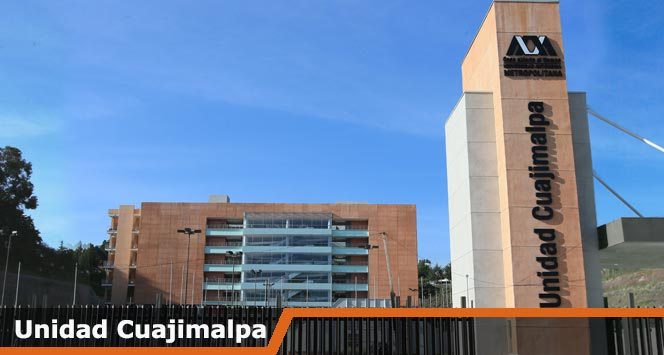
\includegraphics[width=\paperwidth,height=\paperheight]{uam/cua_01.jpg}}
	\begin{frame}[billede]
		\begin{textblock*}{\textwidth}(0\textwidth,0.77\textheight)
			\begin{beamercolorbox}[wd=7.8cm,sep=0.3cm]{rodbox}
				{\huge ¡Gracias!}
			\end{beamercolorbox}
		\end{textblock*}
	\end{frame}
}

%%%%% THIS IS THE BLOCK OF REFERENCES 

% \begin{frame}[hvid, allowframebreaks]
	% \frametitle{Referencias}
	% \printbibliography
	
	% \end{frame}


%%%%%% END OF THE BLOCK OF REFERENCES

\end{document}
